%%%%%%%%%%%%%%%%%%%%%%%%%%%%%%%%%%%%%%%%%%%%%%%%%%%%%%%%%%%%%%%%%%%%%%%%%%%%%%%%
%%%%%%%%%%%%%%%%%%%%%%%%%%%%%%%%%%%%%%%%%%%%%%%%%%%%%%%%%%%%%%%%%%%%%%%%%%%%%%%%
%%                                                                            %%
%% thesistemplate.tex version 3.20 (2018/08/31)                               %%
%% The LaTeX template file to be used with the aaltothesis.sty (version 3.20) %%
%% style file.                                                                %%
%% This package requires pdfx.sty v. 1.5.84 (2017/05/18) or newer.            %%
%%                                                                            %%
%% This is licensed under the terms of the MIT license below.                 %%
%%                                                                            %%
%% Written by Luis R.J. Costa.                                                %%
%% Currently developed at the Learning Services of Aalto University School of %%
%% Electrical Engineering by Luis R.J. Costa since May 2017.                  %%
%%                                                                            %%
%% Copyright 2017-2018, by Luis R.J. Costa, luis.costa@aalto.fi,              %%
%% Copyright 2017-2018 Swedish translations in aaltothesis.cls by Elisabeth   %%
%% Nyberg, elisabeth.nyberg@aalto.fi and Henrik Wallén,                       %%
%% henrik.wallen@aalto.fi.                                                    %%
%% Copyright 2017-2018 Finnish documentation in the template opinnatepohja.tex%%
%% by Perttu Puska, perttu.puska@aalto.fi, and Luis R.J. Costa.               %%
%% Copyright 2018 English template thesistemplate.tex by Luis R.J. Costa.     %%
%% Copyright 2018 Swedish template kandidatarbetsbotten.tex by Henrik Wallen. %%
%%                                                                            %%
%% Permission is hereby granted, free of charge, to any person obtaining a    %%
%% copy of this software and associated documentation files (the "Software"), %%
%% to deal in the Software without restriction, including without limitation  %%
%% the rights to use, copy, modify, merge, publish, distribute, sublicense,   %%
%% and/or sell copies of the Software, and to permit persons to whom the      %%
%% Software is furnished to do so, subject to the following conditions:       %%
%% The above copyright notice and this permission notice shall be included in %%
%% all copies or substantial portions of the Software.                        %%
%% THE SOFTWARE IS PROVIDED "AS IS", WITHOUT WARRANTY OF ANY KIND, EXPRESS OR %%
%% IMPLIED, INCLUDING BUT NOT LIMITED TO THE WARRANTIES OF MERCHANTABILITY,   %%
%% FITNESS FOR A PARTICULAR PURPOSE AND NONINFRINGEMENT. IN NO EVENT SHALL    %%
%% THE AUTHORS OR COPYRIGHT HOLDERS BE LIABLE FOR ANY CLAIM, DAMAGES OR OTHER %%
%% LIABILITY, WHETHER IN AN ACTION OF CONTRACT, TORT OR OTHERWISE, ARISING    %%
%% FROM, OUT OF OR IN CONNECTION WITH THE SOFTWARE OR THE USE OR OTHER        %%
%% DEALINGS IN THE SOFTWARE.                                                  %%
%%                                                                            %%
%%                                                                            %%
%%%%%%%%%%%%%%%%%%%%%%%%%%%%%%%%%%%%%%%%%%%%%%%%%%%%%%%%%%%%%%%%%%%%%%%%%%%%%%%%
%%                                                                            %%
%%                                                                            %%
%% An example for writting your thesis using LaTeX                            %%
%% Original version and development work by Luis Costa, changes to the text   %% 
%% in the Finnish template by Perttu Puska.                                   %%
%% Support for Swedish added 15092014                                         %%
%% PDF/A-b support added on 15092017                                          %%
%% PDF/A-2 support added on 24042018                                          %%
%%                                                                            %%
%% This example consists of the files                                         %%
%%         thesistemplate.tex (version 3.20) (for text in English)            %%
%%         opinnaytepohja.tex (version 3.20) (for text in Finnish)            %%
%%         kandidatarbetsbotten.tex (version 1.00) (for text in Swedish)      %%
%%         aaltothesis.cls (versio 3.20)                                      %%
%%         kuva1.eps (graphics file)                                          %%
%%         kuva2.eps (graphics file)                                          %%
%%         kuva1.jpg (graphics file)                                          %%
%%         kuva2.jpg (graphics file)                                          %%
%%         kuva1.png (graphics file)                                          %%
%%         kuva2.png (graphics file)                                          %%
%%         kuva1.pdf (graphics file)                                          %%
%%         kuva2.pdf (graphics file)                                          %%
%%                                                                            %%
%%                                                                            %%
%% Typeset in Linux either with                                               %%
%% pdflatex: (recommended method)                                             %%
%%             $ pdflatex thesistemplate                                      %%
%%             $ pdflatex thesistemplate                                      %%
%%                                                                            %%
%%   The result is the file thesistemplate.pdf that is PDF/A compliant, if    %%
%%   you have chosen the proper \documenclass options (see comments below)    %%
%%   and your included graphics files have no problems.
%%                                                                            %%
%% Or                                                                         %%
%% latex: (this method is not recommended)                                    %%
%%             $ latex thesistemplate                                         %%
%%             $ latex thesistemplate                                         %%
%%                                                                            %%
%%   The result is the file thesistemplate.dvi, which is converted to ps      %%
%%   format as follows:                                                       %%
%%                                                                            %%
%%             $ dvips thesistemplate -o                                      %%
%%                                                                            %%
%%   and then to pdf as follows:                                              %%
%%                                                                            %%
%%             $ ps2pdf thesistemplate.ps                                     %%
%%                                                                            %%
%%   This pdf file is not PDF/A compliant. You must must make it so using,    %%
%%   e.g., Acrobat Pro or PDF-XChange.                                        %%
%%                                                                            %%
%%                                                                            %%
%% Explanatory comments in this example begin with the characters %%, and     %%
%% changes that the user can make with the character %                        %%
%%                                                                            %%
%%%%%%%%%%%%%%%%%%%%%%%%%%%%%%%%%%%%%%%%%%%%%%%%%%%%%%%%%%%%%%%%%%%%%%%%%%%%%%%%
%%%%%%%%%%%%%%%%%%%%%%%%%%%%%%%%%%%%%%%%%%%%%%%%%%%%%%%%%%%%%%%%%%%%%%%%%%%%%%%%
%%
%% WHAT is PDF/A
%%
%% PDF/A is the ISO-standardized version of the pdf. The standard's goal is to
%% ensure that he file is reproducable even after a long time. PDF/A differs
%% from pdf in that it allows only those pdf features that support long-term
%% archiving of a file. For example, PDF/A requires that all used fonts are
%% embedded in the file, whereas a normal pdf can contain only a link to the
%% fonts in the system of the reader of the file. PDF/A also requires, among
%% other things, data on colour definition and the encryption used.
%% Currently three PDF/A standards exist:
%% PDF/A-1: based on PDF 1.4, standard ISO19005-1, published in 2005.
%%          Includes all the requirements essential for long-term archiving.
%% PDF/A-2: based on PDF 1.7, standard ISO19005-2, published in 2011.
%%          In addition to the above, it supports embedding of OpenType fonts,
%%          transparency in the colour definition and digital signatures.
%% PDF/A-3: based on PDF 1.7, standard ISO19005-3, published in 2012.
%%          Differs from the above only in that it allows embedding of files in
%%          any format (e.g., xml, csv, cad, spreadsheet or wordprocessing
%%          formats) into the pdf file.
%% PDF/A-1 files are not necessarily PDF/A-2 -compatible and PDF/A-2 are not
%% necessarily PDF/A-1 -compatible.
%% All of the above PDF/A standards have two levels:
%% b: (basic) requires that the visual appearance of the document is reliably
%%    reproduceable.
%% a (accessible) in addition to the b-level requirements, specifies how
%%   accessible the pdf file is to assistive software, say, for the physically
%%   impaired.
%% For more details on PDF/A, see, e.g., https://en.wikipedia.org/wiki/PDF/A
%%
%%
%% WHICH PDF/A standard should my thesis conform to?
%%
%% Primarily to the PDF/A-1b standard. All the figures and graphs typically
%% use in thesis work do not require transparency features, a basic '2-D'
%% visualisation suffices. The font to be used are specified in this template
%% and they should not be changed. However, if you have figures where
%% transparency characteristics matter, use the PDF/A-2b standard. Do not use
%% the PDF/A-3b standard for your thesis.
%%
%%
%% WHAT graphics format can I use to produce my PDF/A compliant file?
%%
%% When using pdflatex to compile your work, use jpg, png or pdf files. You may
%% have PDF/A compliance problems with figures in pdf format. Do not use PDF/A
%% compliant graphics files.
%% If you decide to use latex to compile your work, the only acceptable file
%% format for your figure is eps. DO NOT use the ps format for your figures.

%% USE one of these:
%% * the first when using pdflatex, which directly typesets your document in the
%%   chosen pdf/a format and you want to publish your thesis online,

%% * the second when you want to print your thesis to bind it, or
%% * the third when producing a ps file and a pdf/a from it.
%%
\documentclass[english, 12pt, a4paper, elec, utf8, a-1b, online]{aaltothesis}
%\documentclass[english, 12pt, a4paper, elec, utf8, a-1b]{aaltothesis}
%\documentclass[english, 12pt, a4paper, elec, dvips, online]{aaltothesis}

%% Use the following options in the \documentclass macro above:
%% your school: arts, biz, chem, elec, eng, sci
%% the character encoding scheme used by your editor: utf8, latin1
%% thesis language: english, finnish, swedish
%% make an archiveable PDF/A-1b or PDF/A-2b compliant file: a-1b, a-2b
%%                    (with pdflatex, a normal pdf containing metadata is
%%                     produced without the a-*b option)
%% typeset in symmetric layout and blue hypertext for online publication: online
%%            (no option is the default, resulting in a wide margin on the
%%             binding side of the page and black hypertext)
%% two-sided printing: twoside (default is one-sided printing)
%%

%% Use one of these if you write in Finnish (see the Finnish template
%% opinnaytepohja.tex)
%\documentclass[finnish, 12pt, a4paper, elec, utf8, a-1b, online]{aaltothesis}
%\documentclass[finnish, 12pt, a4paper, elec, utf8, a-1b]{aaltothesis}
%\documentclass[finnish, 12pt, a4paper, elec, dvips, online]{aaltothesis}

%% Packages
\usepackage{graphicx}
%% Graphics path
\graphicspath{{doc/0_figures/}}

%% Math fonts, symbols, and formatting; these are usually needed
\usepackage{amsfonts,amssymb,amsbsy,amsmath,gensymb}
\usepackage{wasysym}

%% Glossaries and acronyms
\usepackage[xindy,acronym,nomain,nopostdot,nogroupskip,nonumberlist,acronymlists={acronym,symbolslist,operatorslist}]{glossaries}
\newglossary[tlg]{symbolslist}{tld}{tdn}{Symbols}
\newglossary[slg]{operatorslist}{syi}{syg}{Operators}
\makenoidxglossaries
\loadglsentries{97_glossary}
\glsaddall
\setlength{\glsdescwidth}{0.88\hsize}
\setglossarysection{subsection}

%% Bibliography
\usepackage[backend=biber,citestyle=ieee,citestyle=numeric-comp]{biblatex}
\usepackage{csquotes}
\addbibresource{doc/thesis/99_references.bib}

\usepackage[binary-units=true]{siunitx}
\usepackage{float}
\usepackage{caption}
\usepackage{subcaption}
\usepackage{tabularx}
\usepackage{colortbl}

\usepackage{dirtree}

%% Change the school field to specify your school if the automatically set name
%% is wrong
% \university{aalto-yliopisto}
% \school{Sähkötekniikan korkeakoulu}

%% Edit to conform to your degree programme
%%
\degreeprogram{Space Science and Technology}
%%

%% Your major
%%
\major{Space Robotics and Automation}
%%

%% Major subject code
%%
\code{ELEC3047}
%%
 
%% Choose one of the three below
%%
%\univdegree{BSc}
\univdegree{MSc}
%\univdegree{Lic}
%%

%% Your name (self explanatory...)
%%
\thesisauthor{Gabriel J\"org Schwarzkopf}
%%

%% Your thesis title comes here and possibly again together with the Finnish or
%% Swedish abstract. Do not hyphenate the title, and avoid writing too long a
%% title. Should LaTeX typeset a long title unsatisfactorily, you mght have to
%% force a linebreak using the \\ control characters.
%% In this case...
%% Remember, the title should not be hyphenated!
%% A possible "and" in the title should not be the last word in the line, it
%% begins the next line.
%% Specify the title again without the linebreak characters in the optional
%% argument in box brackets. This is done because the title is part of the 
%% metadata in the pdf/a file, and the metadata cannot contain linebreaks.
%%
\thesistitle{Title of the thesis}
%\thesistitle[Title of the thesis]{Title of\\ the thesis}
%%

%%
\place{Espoo}
%%

%% The date for the bachelor's thesis is the day it is presented
%%
\date{31.8.2018}
%%

%% Thesis supervisor
%% Note the "\" character in the title after the period and before the space
%% and the following character string.
%% This is because the period is not the end of a sentence after which a
%% slightly longer space follows, but what is desired is a regular interword
%% space.
%%
\supervisor{Prof.\ Jaan Praks}
%%

%% Advisor(s)---two at the most---of the thesis. Check with your supervisor how
%% many official advisors you can have.
%%
\advisor{Dr Andris Slavinskis}
%\advisor{MSc Sarah Scientist}
%%

%% Aaltologo: syntax:
%% \uselogo{aaltoRed|aaltoBlue|aaltoYellow|aaltoGray|aaltoGrayScale}{?|!|''}
%% The logo language is set to be the same as the thesis language.
%%
\uselogo{aaltoRed}{''}
%%

%% The English abstract:
%% All the details (name, title, etc.) on the abstract page appear as specified
%% above.
%% Thesis keywords:
%% Note! The keywords are separated using the \spc macro
%%
\keywords{For keywords choose\spc concepts that are\spc central to your\spc thesis}
%%

%% The abstract text. This text is included in the metadata of the pdf file as well
%% as the abstract page.
%%
\thesisabstract{
Your abstract in English. Keep the abstract short. The abstract explains your 
research topic, the methods you have used, and the results you obtained. In the 
PDF/A format of this thesis, in addition to the abstract page, the abstract text is 
written into the pdf file's metadata. Write here the text that goes into the 
metadata. The metadata cannot contain special characters, linebreak or paragraph 
break characters, so these must not be used here. If your abstract does not contain 
special characters and it does not require paragraphs, you may take advantage of 
the abstracttext macro (see the comment below). Otherwise, the metadata abstract 
text must be identical to the text on the abstract page.
}

%% Copyright text. Copyright of a work is with the creator/author of the work
%% regardless of whether the copyright mark is explicitly in the work or not.
%% You may, if you wish, publish your work under a Creative Commons license (see
%% creaticecommons.org), in which case the license text must be visible in the
%% work. Write here the copyright text you want. It is written into the metadata
%% of the pdf file as well.
%% Syntax:
%% \copyrigthtext{metadata text}{text visible on the page}
%% 
%% In the macro below, the text written in the metadata must have a \noexpand
%% macro before the \copyright special character, and macros (\copyright and
%% \year here) must be separated by the \ character (space chacter) from the
%% text that follows. The macros in the argument of the \copyrighttext macro
%% automatically insert the year and the author's name. (Note! \ThesisAuthor is
%% an internal macro of the aaltothesis.cls class file).
%% Of course, the same text could have simply been written as
%% \copyrighttext{Copyright \noexpand\copyright\ 2018 Eddie Engineer}
%% {Copyright \copyright{} 2018 Eddie Engineer}
%%
\copyrighttext{Copyright \noexpand\copyright\ \number\year\ \ThesisAuthor}
{Copyright \copyright{} \number\year{} \ThesisAuthor}

%% You can prevent LaTeX from writing into the xmpdata file (it contains all the 
%% metadata to be written into the pdf file) by setting the writexmpdata switch
%% to 'false'. This allows you to write the metadata in the correct format
%% directly into the file thesistemplate.xmpdata.
%\setboolean{writexmpdatafile}{false}



%% All that is printed on paper starts here
%%
\begin{document}

%% Create the coverpage
%%
\makecoverpage

%% Typeset the copyright text.
%% If you wish, you may leave out the copyright text from the human-readable
%% page of the pdf file. This may seem like a attractive idea for the printed
%% document especially if "Copyright (c) yyyy Eddie Engineer" is the only text
%% on the page. However, the recommendation is to print this copyright text.
%%
\makecopyrightpage

%% Note that when writting your thesis in English, place the English abstract
%% first followed by the possible Finnish or Swedish abstract.

%% Abstract text
%% All the details (name, title, etc.) on the abstract page appear as specified
%% above.
%%
% \begin{abstractpage}[english]
%   Your abstract in English. Keep the abstract short. The abstract explains your
%   research topic, the methods you have used, and the results you obtained.  
  
%   The abstract text of this thesis is written on the readable abstract page as
%   well as into the pdf file's metadata via the $\backslash$thesisabstract macro
%   (see above). Write here the text that goes onto the readable abstract page.
%   You can have special characters, linebreaks, and paragraphs here. Otherwise,
%   this abstract text must be identical to the metadata abstract text.
  
%   If your abstract does not contain special characters and it does not require
%   paragraphs, you may take advantage of the abstracttext macro (see the comment
%   below).
% \end{abstractpage}

%% The text in the \thesisabstract macro is stored in the macro \abstractext, so
%% you can use the text metadata abstract directly as follows:
%%
\begin{abstractpage}[english]
	\abstracttext{}
\end{abstractpage}

%% Preface
%%
%% This section is optional. Remove it if you do not want a preface.
\mysection{Preface}
%\mysection{Esipuhe}
I want to thank Professor Jaan Praks and my instructor Andris Slavinskis, PhD for 
their good and poor guidance.\\

\vspace{5cm}
Otaniemi, 31.8.2018

\vspace{5mm}
{\hfill \ThesisAuthor \hspace{1cm}}

%% Force a new page after the preface
%%
\newpage


%% Table of contents. 
%%
\thesistableofcontents


%% Symbols and abbreviations
\mysection{Symbols and abbreviations}

\printnoidxglossary[type=symbolslist, style=long]

\printnoidxglossary[type=operatorslist, style=long]

\printnoidxglossary[type=\acronymtype, style=long, title={Abbreviations}] 

%% \clearpage is similar to \newpage, but it also flushes the floats (figures
%% and tables).
%%
\cleardoublepage

%% Text body begins. Note that since the text body is mostly in Finnish the
%% majority of comments are also in Finnish after this point. There is no point
%% in explaining Finnish-language specific thesis conventions in English.
%% This text will be translated to English soon.
%%
\section{Introduction}
\section{Introduction}
Studying \gls{sssb}s is getting more and more interesting. There are several aspects to this. From a scientific perspective, \gls{sssb}s are interesting, because they are unaltered remnants from the formation of the Solar System. Economically, \gls{sssb} are becoming interesting, as there are several materials that could be mined from them. Thirdly, planetary defence is interested in defending Earth from a possible threat by \gls{sssb}.

Currently, there is only a very limited knowledge on \gls{sssb} available. Most knowledge about there size, shape and colour is inferred from ground based observations and space telescopes. Another method is close-up observation through spacecraft. Only {\color{red}XXX} bodies have been visited by spacecraft, either with a fly-by {\color{red}(XXX)} or going into orbit around them {\color{red}(XXX)}. Considering the approx. ~{\color{red} XXXXXXX} known bodies shows how many more objects there are to be discovered. Whilst it is possible to obtain a rough overall statistics of many \gls{sssb}s using ground and space telescopes, fly-by and missions going into orbit around an \gls{sssb} can provide a much more detailed analysis of these bodies through in-situ measurements and showing local variations of e.g. albedo.

Advancing the field requires improving the statistics on the different types of \gls{sssb}s \cite{Pajusalu2019CharacterizationMapping}. Several new mission ideas are aiming for this goal. However, technological challenges have to be overcome first. Additionally, new mission concepts like the \gls{ci} mission require a new approach to model \gls{sssb}s. \gls{ci} is a mission that will investigate either a dynamically new comet from the Öpik-Oort cloud or an interstellar object. The mission will consist of a main spacecraft and two sub-spacecrafts that will be launched to the \gls{l2} and wait until a suitable \gls{sssb} will pass by. Consequently, the target body will not be known before launch hence systems have to be developed to deal with a large variety of bodies. However, only few \gls{sssb}s have been visited by spacecraft and thus only very limited real images are available. A method to deal with such sparse available data is to synthetically create images of \gls{sssb}s.

Miniaturisation of technology enables completely new types of missions. With increasing capabilities of smaller spacecraft, they are becoming more and more considered for deep space missions. Either in mother-daughter spacecraft combinations (comet interceptor) or as swarms of satellites (MAT). Small satellites not only increase the number of spacecraft but also allow for probing more dangerous environments due to the decreased costs. However, this increase in deep space missions requires new methods for navigation and data transmission due to limited data budgets. Currently, all missions rely on a \gls{dsn} for both functions. The increasing number of spacecraft requires an increasing level of on-board autonomy in both, navigation and data compression for communication.

One step towards higher on-board autonomy is the prioritisation of images for transmission. With the  possibility of loss of spacecraft during proximity operations, the most relevant information needs to be transmitted first and later complemented with additional data if possible.

Furthermore, to increase navigation autonomy on-board deep space missions, optical navigation will be used for proximity operations. One problem in developing such system is the limited number and availability of real images. To solve this problem synthetic image generation can be used.

Within this work, the \gls{sispo} was developed. This simulation environment allows to create different 3D models of \gls{sssb}s using procedural surface generation. This approach allows to create different surface textures as well as different shapes for \gls{sssb}. These models can then be used to render photo-realistic images for a given \gls{sssb} orbit and spacecraft trajectory. Current methods mostly rely on an approximation to render e.g. the shadows on \gls{sssb}s. The proposed approach uses ray-tracing to generate photo-realistic images.

As a second part, \gls{sispo} can reconstruct 3D models from images via a \gls{sfm} approach. Since the data budget of small satellite missions is heavily limited, and there is a high risk of losing such a spacecraft due to the higher risk environments, maximising the science output becomes a problem of data compression and transmission. 
This thesis focuses on image compression and decompression. These effects will be quantified using the reconstructed 3D models against the "ideal" model. A reference instrument definition similar to a suggested instrument for the 'Comet Interceptor' mission. Different compression and decompression algorithms will be evaluated using different \gls{sssb}s. Furthermore, different spacecraft trajectories will be examined to investigate limitations of the simulation environment.

%% Leave page number of the first page empty
%% 
\thispagestyle{empty}


%% In a thesis, every section starts a new page, hence \clearpage
\clearpage

\section{Background}
\section{Background}
Notes
\gls{nasa} is interested in topic\\
autoNGC\\

Compression types:
    - \gls{dct}
    - Wavelet transform
    - Fractal compression
    - AI based image compression?
    - 

%% Three levels of hierarchy in sectioning should be enough

\subsection*{Numerointi}

Every section of the thesis begins on a new page. A subsection begins on a new 
page only if the previous page a full.

The page numbering begins from the cover page and it is continuous through to 
the end. Arabian numerals are in the page numbering.

The page numbers are made visibleafter the abstract pages, from the preface 
onwards, if there is one, or from the table of contents onwards.

The list of references (bibliography) begins on a new page.

Every appendix begins on a new page. Its page number continues from that on the
previous page.

The page number is place on the upper corner of the page.

%% The example for embedding the graphics file linediagram.pdf into the document.
%% Command \inclugraphics[parametres]{argument} embeds the graphic.
%% Command \centering centres the graphic on the page horizontally. 
%% Command \caption numbers and places the caption at the position of occurrence.
%% Parameters htb force the figure to the current place of occurrence in the
%% source file, if there is sufficient space, or places it to the top or bottom
%% of the page. 
%\begin{figure}[htb]
%\centering
%% NOTE! The PDF/A-1b file created when using the jpg, pdf or png file below is
%% error-free. However, with kuva1.pdf, the resulting PDF/A-2b file fails the
%% compliance test in Acrobat Pro but passes it in PDF-XChanger and the validator
%% at https://www.pdf-online.com/osa/validate.aspx tarkistuksen.
%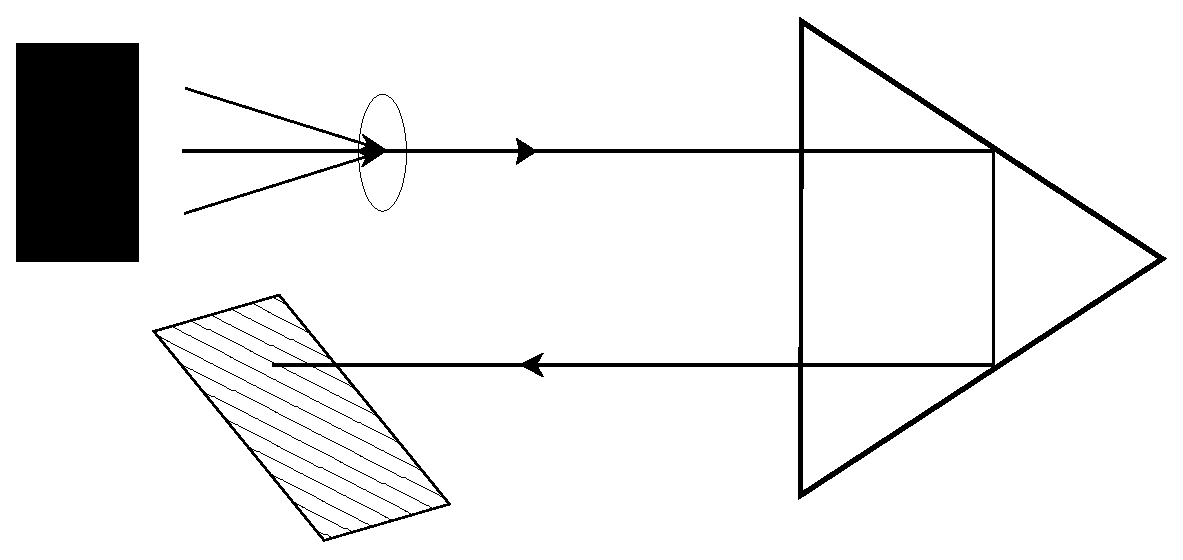
\includegraphics[height=5cm]{linediagram.eps}
%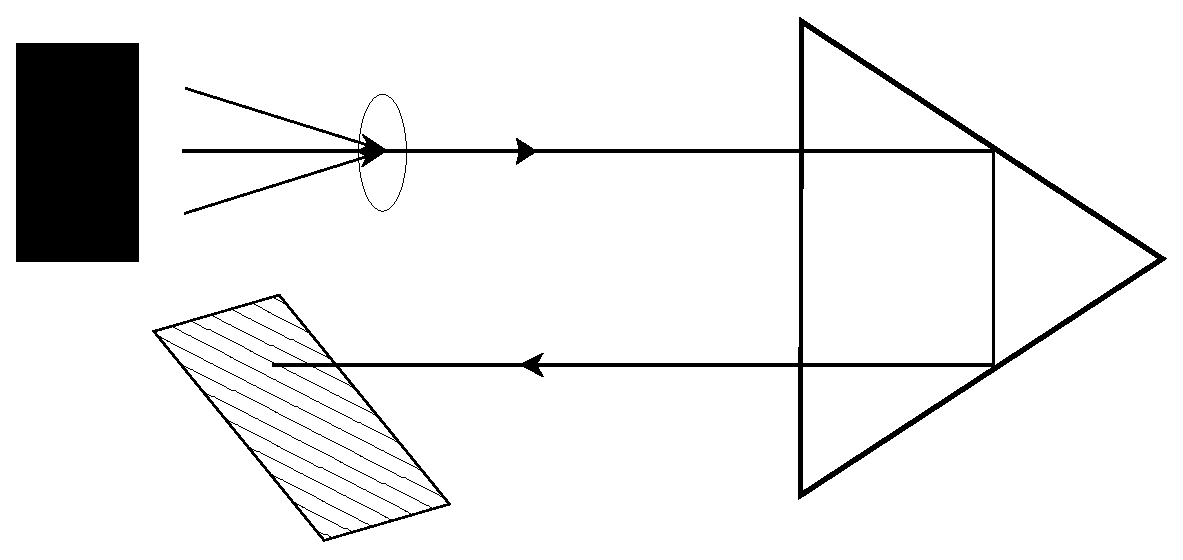
\includegraphics[height=5cm]{./linediagram.eps}
%\caption{This is an example of a numbered caption. \label{kuva1}}
%\end{figure}

% \begin{figure}[htb]
% \centering
% 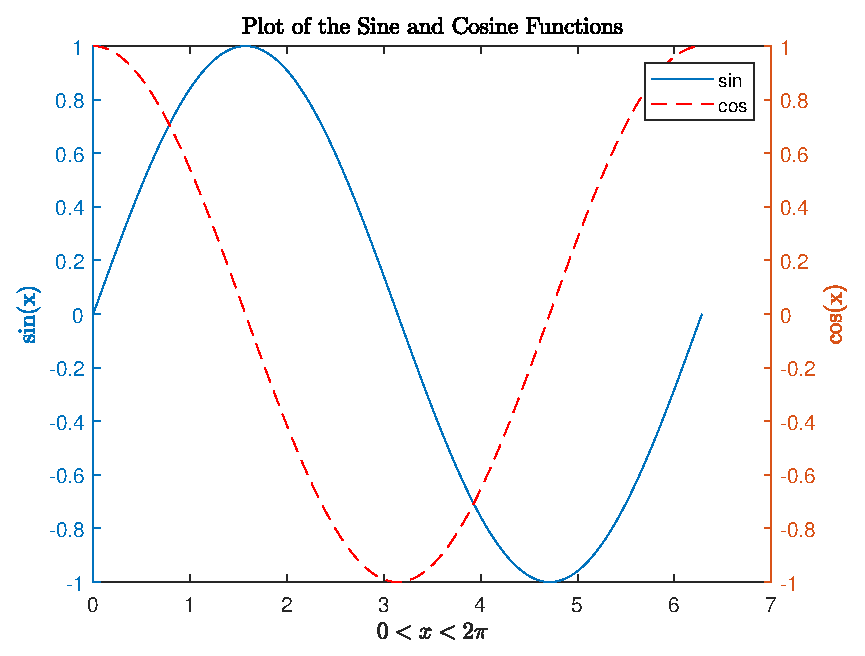
\includegraphics[height=5cm]{curves.eps}
% %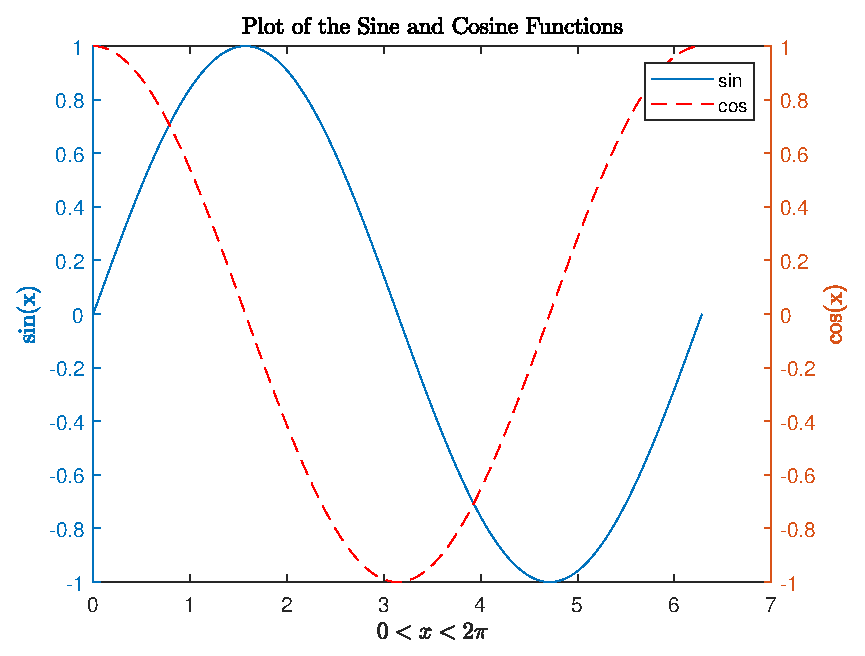
\includegraphics[height=5cm]{curves.eps}
% \caption{This is an example of a MATLAB graph. \label{kuva2}}
% \end{figure}


\clearpage

\section{Research material and methods}
%\section{Tutkimusaineisto ja -menetelm\"at}


\clearpage

\section{Results}
%\section{Tulokset}



\clearpage

\section{Summary} 
%\section{Yhteenveto}


\clearpage
%% L\"ahdeluettelo

\thesisbibliography
\printbibliography
%\bibliographystyle{plain}
%\begin{thebibliography}{99}
%\bibliographystyle{ieeetr}
%\bibliography{99_references}
%\end{thebibliography}

%% Appendices
%% If you don't have appendices, remove \clearpage and \thesisappendix below.
\clearpage

\thesisappendix

\section{Esimerkki liitteest\"a\label{LiiteA}}


Liitteet eiv\"at ole opinn\"aytteen kannalta v\"altt\"am\"att\"omi\"a ja 
opinn\"aytteen tekij\"an on 
kirjoittamaan ryhtyess\"a\"an hyv\"a ajatella p\"arj\"a\"av\"ans\"a ilman liitteit\"a.
Kokemattomat kirjoittajat, jotka ovat huolissaan
tekstiosan pituudesta, paisuttavat turhan 
helposti liitteit\"a pit\"a\"akseen tekstiosan pituuden annetuissa rajoissa.
T\"all\"a tavalla ei synny hyv\"a\"a opinn\"aytett\"a.   

Liite on itsen\"ainen kokonaisuus, vaikka se t\"aydent\"a\"akin tekstiosaa.
Liite ei siten ole pelkk\"a listaus, kuva tai taulukko, vaan 
liitteess\"a selitet\"a\"an aina sis\"all\"on laatu ja tarkoitus. 

Liitteeseen voi laittaa esimerkiksi listauksia. Alla on 
listausesimerkki t\"am\"an liitteen luomisesta. 

%% Verbatim-ymp\"arist\"o ei muotoile tai tavuta teksti\"a. Fontti on monospace.
%% Verbatim-ymp\"arist\"on sis\"all\"a annettuja komentoja ei LaTeX k\"asittele. 
%% Vasta \end{verbatim}-komennon j\"alkeen jatketaan k\"asittely\"a.
\begin{verbatim}
	\clearpage
	\appendix
	\addcontentsline{toc}{section}{Liite A}
	\section*{Liite A}
	...
	\thispagestyle{empty}
	...
	teksti\"a
	...
	\clearpage
\end{verbatim}

Kaavojen numerointi muodostaa liitteiss\"a oman kokonaisuutensa:
\begin{align}
d \wedge A &= F, \label{liitekaava1}\\
d \wedge F &= 0. \label{liitekaava2}
\end{align}


\clearpage
\section{Toinen esimerkki liitteest\"a\label{LiiteB}}

%% Liitteiden kaavat, taulukot ja kuvat numeroidaan omana kokonaisuutenaan
%%
%% Equations, tables and figures have their own numbering in Appendices
%\renewcommand{\theequation}{B\arabic{equation}}
%\setcounter{equation}{0}  
%\renewcommand{\thefigure}{B\arabic{figure}}
%\setcounter{figure}{0}
%\renewcommand{\thetable}{B\arabic{table}}
%\setcounter{table}{0}

Liitteiss\"a voi my\"os olla kuvia, jotka
eiv\"at sovi leip\"atekstin joukkoon:
%% Ymp\"arist\"on figure parametrit htb pakottavat
%% kuvan t\"ah\"an, eik\"a LaTeX yrit\"a siirrell\"a niit\"a
%% hyv\"aksi katsomaansa paikkaan. 
%% Ymp\"arist\"o\"a center voi k\"aytt\"a\"a \centering-
%% komennon sijaan
%%
%% Example of a figure, note the use of htb parameters which force
%% the figure to be inserted here
\begin{figure}[htb]
\begin{center}
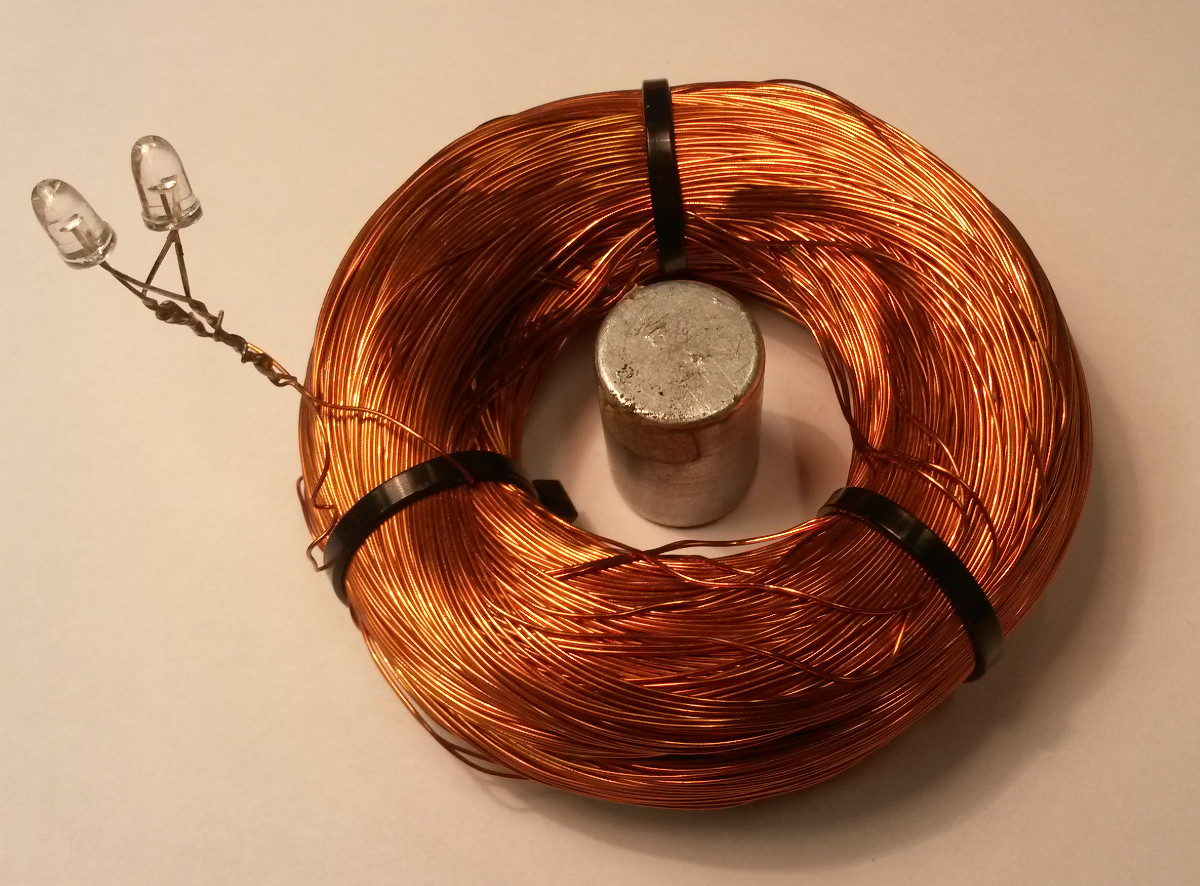
\includegraphics[height=8cm]{ledspole.jpg}
\end{center}
\caption{Kuvateksti, jossa on liitteen numerointi}
\label{liitekuva}
\end{figure}
%%
Liitteiden taulukoiden numerointi on kuvien ja kaavojen kaltainen:
\begin{table}[htb]
\caption{Taulukon kuvateksti.}
\label{liitetaulukko}
\begin{center}
\fbox{
\begin{tabular}{lp{0.5\linewidth}}
9.00--9.55  & K\"aytett\"avyystestauksen tiedotustilaisuus (osanottajat
ovat saaneet s\"ahk\"opostitse valmistautumisteht\"av\"at, joten tiedotustilaisuus
voidaan pit\"a\"a lyhyen\"a).\\
9.55--10.00 & Testausalueelle siirtyminen
\end{tabular}}
\end{center}
\end{table}
Kaavojen numerointi muodostaa liitteiss\"a oman kokonaisuutensa:
\begin{align}
T_{ik} &= -p g_{ik} + w u_i u_k + \tau_{ik},  \label{liitekaava3} \\
n_i    &= n u_i + v_i.                      \label{liitekaava4}
\end{align}

\end{document}
